% \hspace{10pt}
Nesta primeira tarefa deverão ser aprendidos conhecimentos de simulação de parâmetros do circuito e transistor (ponto de operação e valores de tensão e corrente nas malhas do circuito). Além disso, esse é o laboratório em que você deverá desenvolver suas habilidades no software de simulação de circuitos.

Antes de começar tenha certeza de que você assistiu os vídeos de introdução e configuração do software no ambiente da UFPB. A configuração do ambiente não faz parte desse roteiro. Para dar início ao roteiro, abra o virtuoso com a tecnologia TSMC180nm configurada e crie uma nova biblioteca {\em lab01} que deverá conter todas as células de circuitos e simulações dessa tarefa.

Dentro da biblioteca {\em lab01} crie uma nova célula chamada {\em transistor\_dc\_param}. É à partir dessa célula que você deverá efetuar as primeiras simulações para encontrar os parâmetros do transistor. Na célula, crie o circuito de acordo com a Figura~\ref{circuito}.
\begin{figure}[hbt!]
  \centering
    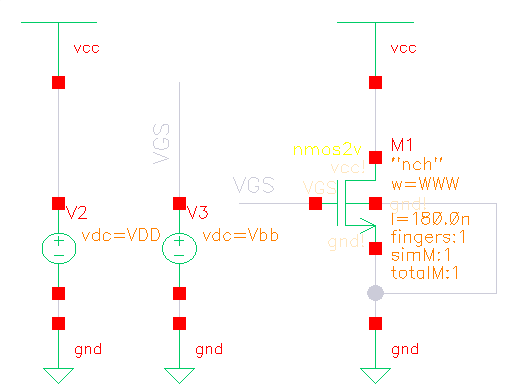
\includegraphics[width=0.6\textwidth]{transistor_dc_sim.png}
    \caption{Circuito 01.\label{circuito}}
\end{figure}

\newpage
Você irá precisar de:
\begin{enumerate}
    \item {\em tsmc18} tech:
    \begin{enumerate}
        \item Transistor NMOS: nmos2v
    \end{enumerate}
    \item {\em analogLib}:
    \begin{enumerate}
        \item Voltage Source: 2x vdc
        \begin{enumerate}
            \item VDD = 2 V
            \item Vbb = 1 V
        \end{enumerate}
        \item Voltage Sourcel 2x vcc
        \item Voltage Source: 3x gnd
    \end{enumerate}
\end{enumerate}

Após salvar a visão esquemático da célula (lembre-se de utilizar o botão {\em check-and-save}), você deverá lançar o simulador de circuitos. Para isso vá até {\em Launch$\rightarrow$ADE} L na janela do virtuoso onde está seu esquemático. A simulação DC é selecionada pelo menu {\em Analysis$\rightarrow$Choose$\rightarrow$DC}. Selecione a opção {\em Save DC operating point} e clique OK.

\noindent Após o término do {\em setup} básico de simulações, responda:

%%% -- Questão 01 - 6.24
\begin{questions}
\question Qual o valor da tensão Vth do transistor na configuração padrão\footnote{{\em Padrão} significa que você não alterou nenhum parâmetro do transistor}? 
\begin{EnvFullwidth}
\makeemptybox{1in}
\end{EnvFullwidth}
\question A tensão $V_{TH}$ modifica com a variação do tamanho do transistor? Faça variar W e faça um plot paramétrico entre $W$ vs. $V_{TH}$. Para isso, será preciso que você modifique o parâmetro $W$ do transistor e em simulação varie o tamanho de $W$. Utilize os seguintes valores para a simulação paramétrica:
\begin{itemize}
    \item variable: W
    \item from: 2u
    \item to: 200u
    \item step-mode: decade
    \item step-decade: 10
\end{itemize}
 O que acontece (adicione o print do gráfico de resposta em uma folha em anexo)? Explique (pesquise a resposta).
\begin{EnvFullwidth}
\makeemptybox{2in}
\end{EnvFullwidth}
\newpage
{\em cont.}
\begin{EnvFullwidth}
\makeemptybox{4in}
\end{EnvFullwidth}
\question Modifique os valores do transistor para que ele tenha $L=180nm$ e $W=10\mu m$ e simule a curva característica do transistor para 0$\leq$V\textsubscript{DD}$\leq$2 e 0.3$\leq$V\textsubscript{BB}$\leq$1.2. 
Para isso será preciso que:
\begin{enumerate}
    \item Modifique o parâmetro {\em tensão DC} da fonte V3 ({\em gate}) da Figura~\ref{circuito} para uma variável ({\em vgs}, por exemplo) a ser modificada pelo simulador.
    \item Nos parâmetros de simulação DC 
    \begin{enumerate}
        \item selecione a opção {\em Sweep variable$\rightarrow$Component Parameter$\rightarrow$Select Component}, selecione a fonte de tensão de porta e por fim o parâmetro {\em dc}, que é o valor de tensão dc da fonte.
        \item Na opção {\em Sweep Range:}
            \begin{itemize}
                \item select {\em start-stop}
                \item start: 0
                \item to: 2
                \item step-mode: linear
                \item number of points: 101
            \end{itemize}    
        \end{enumerate}
    \item Selecione {\em Tools$\rightarrow$ Parametric Analysis} e coloque os valores para simulação para variação da tensão V\textsubscript{GS}:
        \begin{itemize}
            \item variable: {\em vgs}
            \item from: 0.3
            \item to: 1.2
            \item step-mode: linear
            \item mumber of points: 10
        \end{itemize}
\end{enumerate}
Após simular, adicione o print do gráfico de resposta em anexo e responda as seguintes perguntas:
\begin{parts}
\part Se VCC = 1.1V e Vb = 0.9 V, responda:
\begin{enumerate}
    \item Qual é a corrente do transistor?
    \item É possível avaliar pelo gráfico em que região de operação o transistor está operando quando VCC = 1.1V e Vb = 0.9 V? Se sim, qual é sua região de operação? Justifique.
    \item Qual o ganho de transcondutância {\em gm} do transistor?
\end{enumerate}
\makeemptybox{5in}
\part Com base nos resultados gráficos obtidos em simulação, encontre qual o valor de $\mu_nC_{ox}$ para essa tecnologia. Utilize a equação característica do transistor.
\makeemptybox{3in}
\end{parts}
\end{questions}

%colocar um item para encontrar o valor aproximado de uncox por uma simulação DC de polarização.